\documentclass[11pt]{beamer}
\usetheme{Rochester}
\usepackage[utf8]{inputenc}
\usepackage[francais]{babel}
\usepackage[T1]{fontenc}
\usepackage{amsmath}
\usepackage{amsfonts}
\usepackage{amssymb}
\usepackage{tikz}

\author{Brachet Matthieu}
\title{Modélisation et analyse numérique}
\begin{document}

\begin{frame}
\titlepage
\end{frame}

%% ***************************************************************

\begin{frame}{Enigme}
\begin{columns}
\column{0.45\textwidth}
\begin{center}
\begin{figure}
\includegraphics[scale=0.5]{nenuphare.jpeg}
\end{figure}
\end{center}

\column{0.45\textwidth}
\begin{block}{Petite énigme}
Un nénuphar vit au milieu d'un étang, tous les jours sa surface double. Il a mis 17 jours pour recouvrir la moitié de la surface totale de l'étang. Combien de jours mettra ce même nénuphar pour recouvrir l'intégralité de la surface de l'étang ?
\end{block}

\pause
\begin{flushright}
Réponse : 18 jours.
\end{flushright}
\end{columns}
\end{frame}

%% ***************************************************************

\begin{frame}{et les maths?}
\'Ecriture d'un modèle mathématique :
\begin{center}\textbf{
[Surface demain] $\mathbf{ = 2 \times }$ [Surface aujourd'hui]}
\end{center}

\pause
En langage mathématique :
$$
\mathbf{S_{n+1} = 2 \times S_n}
$$

\pause
\textbf{Problèmes :}
\begin{itemize}
\item Et au bout de 15 jours et 8 heures?
\item Quantité de nourriture pour le nénuphar?
\item Surface de l'étang?
\item ...
\end{itemize}
\end{frame}

%% ***************************************************************

\begin{frame}{Modélisation}

\'Ecriture d'une équation plus complexe, par exemple :
$$
S'(t) = 2 S(t) \times \left( 1 - \dfrac{S(t)}{S_{\text{étang}}} \right)
$$

si je prend en compte la surface de l'étang.

\vspace{1cm}
\pause

\textbf{Si} je connais la fonction $S$, je connais la surface du nénuphar \textbf{en tout temps} !

\pause
\begin{block}{Problème}
Je ne suis pas toujours capable de trouver $S$!
\end{block}

\end{frame}

%% ***************************************************************

\begin{frame}{Modélisation et analyse numérique}

\begin{block}{Modélisation}
\'Ecrire une question réelle avec des maths!
\end{block}

\vspace{1cm}
\pause

\begin{block}{Analyse numérique}
Lorsque je ne sais pas résoudre ce problème : recherche d'une \textbf{solution approchée}.
\end{block}

\end{frame}

%% ***************************************************************

\begin{frame}{Prédiction}

$$S_{n+1}= S_n + \text{évolution}$$

\begin{center}
\begin{tikzpicture}[scale=1]
\draw [>=latex,->] (0,0) -- (8,0);
\draw (0,0) node[below] {0 sec} node{$\bullet$};
\draw (1.5,0) node[below] {5 sec} node{$\bullet$};
\draw (3,0) node[below] {10 sec} node{$\bullet$};
\draw (6,0) node[below] {1 h} node{$\bullet$};
\draw [>=latex,->] (1.5,0.2) arc (180:0:0.75) ;
\end{tikzpicture}
\end{center}
\end{frame}

%% ***************************************************************

\begin{frame}{Deviner la suite}

Un peu comme au cinéma, je veux deviner la suite du film...

\begin{center}
\begin{figure}
\includegraphics[scale=0.25]{film_color.png}
\end{figure}
\end{center}

Ce que je sais :
\begin{itemize}
\item Je regarde un film, \pause
\item C'est un Blockbuster, \pause
\item Film interdit au moins de 16 ans, \pause
\item ...
\end{itemize}

\end{frame}

%% ***************************************************************

\begin{frame}{Ma thèse}
\begin{center}
\textit{Schémas compacts hermitiens sur la sphère - Applications en climatologie et en océanographie numérique.}
\end{center}
Sous la direction de Jean-Pierre Croisille.

Utiliser des méthodes numériques pour résoudre des équations issues du climat.

\begin{block}{Modèle mathématique}
$$
\left\lbrace
\begin{array}{c}
\dfrac{\partial h}{\partial t} = - \nabla \cdot ( h \mathbf{v})\\
\dfrac{\partial \mathbf{v}}{\partial t} + (\mathbf{v} \cdot \nabla) \mathbf{v} + f \mathbf{k} \wedge \mathbf{v} + g \nabla h = 0
\end{array}
\right.
$$
\end{block}
\end{frame}


%% ***************************************************************

\begin{frame}{Maillage}

Je ne peux pas regarder partout et je veux une résolution approchée!

$\Rightarrow$ \textbf{Résolution d'équation issues de la climatologie sur un maillage}

\begin{center}
\begin{figure}
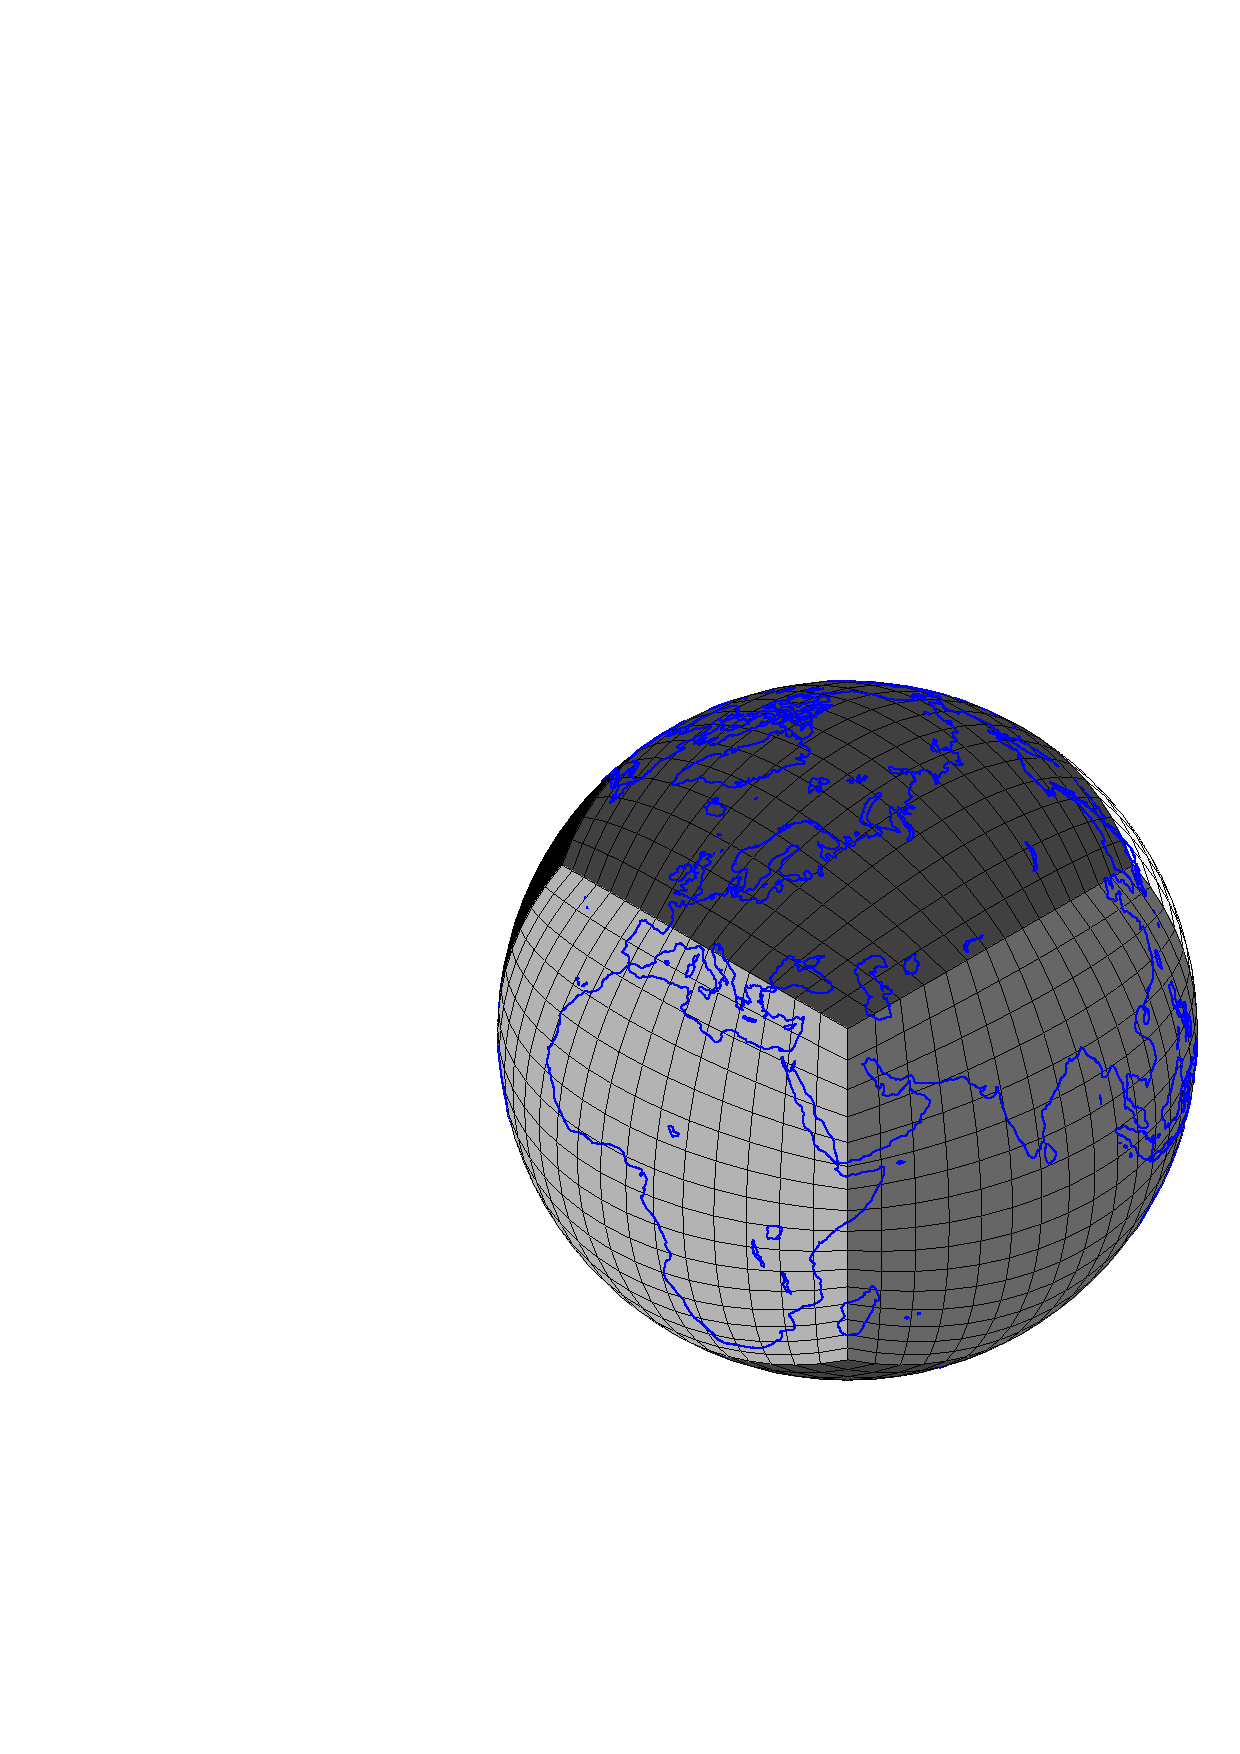
\includegraphics[scale=0.4]{CS.png}
\end{figure}
\end{center}

\end{frame}

%% ***************************************************************

\begin{frame}{Simulations}

Pour valider ma méthode, je l'\textbf{étudie} et je fais des \textbf{tests} sur ordinateur :

\pause
\begin{center}
\begin{figure}
\includegraphics[scale=0.4]{G.png}
\end{figure}
\end{center}

\end{frame}

%% ***************************************************************

\begin{frame}{Simulations}

Pour valider ma méthode, je l'\textbf{étudie} et je fais des \textbf{tests} sur ordinateur :

\begin{center}
\begin{figure}
\includegraphics[scale=0.4]{RH.png}
\end{figure}
\end{center}

\end{frame}

%% ***************************************************************

\begin{frame}{Autres applications :}

\textbf{Imagerie Medicale :}
\begin{center}
\begin{figure}
\includegraphics[scale=0.3]{medic.jpg}
\end{figure}
\end{center}

\end{frame}

%% ***************************************************************

\begin{frame}{Autres applications :}

\textbf{Aviation :}
\begin{center}
\begin{figure}
\includegraphics[scale=0.20]{avion.jpg}
\end{figure}
\end{center}

\end{frame}

%% ***************************************************************

\begin{frame}{Autres applications :}

\textbf{Cinéma :}
\begin{center}
\begin{figure}
\includegraphics[scale=0.15]{vaiana.jpg}
\caption{Film "Vaiana".}
\end{figure}
\end{center}

\end{frame}

%% ***************************************************************

\begin{frame}
\begin{center}
Merci de votre attention :)
\end{center}
\end{frame}



\end{document}